\section{Introduction of the ExtraSensory Dataset}

The ExtraSensory data set was collected in 2015 and 2016 by Yonatan Vaizman and Katherine Ellis under the supervision of Professor Gert Lanckriet. It is based on sensor data from smartphones and smartwatches produced by 60 participants in intervals of one minute. In contrast to many other data sets, the data was generated by normal everyday devices using multiple sensors were in parallel. Furthermore, the participants behavior was not scripted like in many other case studies and they were allowed to behave in an natural way. The sensors included an accelerometer, gyroscope, location and audio sensor and were used by almost everyone in most of the recordings. Additionally some participants used smart watches or fitness tracker which provided an addition watch accelerometer.

The assignment of the data points to activities was mostly done by the users themselves, who had the option to use predefined labels or create their own. In a preprocessing step these label were reduced to a set of 51 labels by combining similar label. The result were 377,346 data points, which were described with one or more of the 51 final labels. The label represent various information about the location, the context and the activity of a user. some examples are 'in class', 'singing', 'stairs (going up)', 'stairs (going down)', 'with friends' or 'talking'.

This means that for each data point a label vector of length 51 exists. Each entry can contain the values true, false or NaN, where NaN represents missing information on this label. The following examination of the data points shows that many labels remained unobserved in each data point:

\begin{figure}[H]
	\begin{center}
		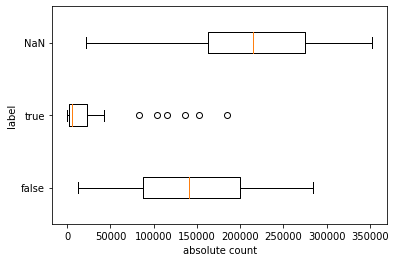
\includegraphics[scale=.8]{images/boxplot_label.png}
		\caption{A box-plot showing the distribution of the absolute count of a given value (false, true or NaN) over the different labels. The yellow line represents the median, the rectangle the 25\% percentile, the line the 75\% percentile and the dotes are outliers.}
		\label{abb:boxplot_label}
	\end{center}		
\end{figure}	

Figure \ref{abb:boxplot_label} visualizes the distribution for each label and a specific value (false, ture or NaN) as a box-plot diagram. Looking at the median for NaN, it can be seen that for most labels the majority of data points do not contain a value - which increases the difficulty of classification. This means that for many labels there is a large number of data points that do not contain any information about the label.

Furthermore, it can be seen that the median labels with the value true is just 5,153 and that only very few labels at all are labeled as true for more than 10\% of the data points. So there are many label classes which contain very few positive representatives. 

\begin{figure}[H]
	\begin{center}
		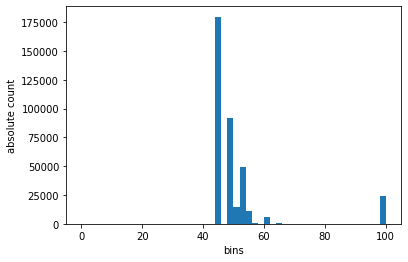
\includegraphics[scale=.8]{images/hist.png}
		\caption{Histogram of absolute counts of percentage of NaN values for each data point. The data is distributed into 50 bins. Each bin has the size of 2 \% of the labels.}
		\label{abb:histogramm_data}
	\end{center}		
\end{figure}

Finally, it can be seen that in all data points at least 44\% of the 51 labels are not evaluated. Thus, there are no data points that make statements about all labels at the same time.